\section{PPO Algorithm}
Με τον αλγόριθμο PPO έγιναν 4 εκαπιδέυσεις:

1. Η εκπαίδευση πραγματοποιήθηκε με CNNPolicy, xωρίς ορίσματα (defaultCNNPolicy).

2. Η εκπαίδευση πραγματοποιήθηκε με CNNPolicy και με όρισμα το CNN μοντέλο (customCNNPolicy).

3. Η εκπαίδευση πραγματοποιήθηκε με MlpPolicy χωρίς ορίσματα (defaultMlpPolicy) .

4. Η εκπαίδευση πραγματοποιήθηκε με MlpPolixy και με όρισμα το NN μοντέλο (customMlpPolicy).


\subsection{Default CNNPolicy vs Custom CNNPolicy}

Στις δύο πρωτες εκπαιδεύσεις έχουν παραχθεί τα παρακάτω 5 διαγράμματα \ref{f:g1}, \ref{f:g2}, \ref{f:g3}, \ref{f:g4} \ref{f:g5}. Το episode/evaluation length διάγραμμα μας εξηγεί πόση ώρα έτρεχε το παιχνιδι, δηλαδή  μπορούμε να καταλάβουμε την διάρκεια που παρέμεινε το αεροπλάνο ζωντανό. Όσο αυξάνεται η διάρκεια του παιχνιδιού παρατηρούμε και άυξηση του reward που παίρνει σε κάθε επεισόδιο ή κατα την evaluation κατασταση.
Tο customCNNPolicy (η πράσινη γραμμή) παρόλο που στο κάθε επεισόδιο παραμένει σχεδόν πάντα πιο πάνω τόσο σto episode length (βλέπε \ref{f:g1}) όσο και στο episode reward (βλέπε \ref{f:g2}), στην evaluation φάση του μοντέλου και στα δύο διαγράμματα στο τέλος πέφτει, ενώ σε όλη την διάρκεια ήταν είτε στο ίδιο επίπεδο με το defaultCNNPolicy είτε λίγο πιο πάνω. Αυτό ίσως συμβαίνει λόγω της ευαισθησίας του CNN μοντέλου στις παραμέτρους που έχουμε βαλει κατα την εκπαίδευση ή απλά είναι ένα τυχαίο γεγονός και άν το συνεχίζαμε να ξανα περνούσε το defaultCNNPolicy. Η δεύτερη περίπτωση φαίνεται πiθανότερη παρατηρόντας το διάγραμμα με το train loss των δύο εκπαιδεύσεων \ref{f:g5}.
Επίσης στο defaultCNNPolicy έχουμε exploration-exploitation trade-off(εξήγηση παρακάτω).




\begin{figure}[ht]
	\centering
	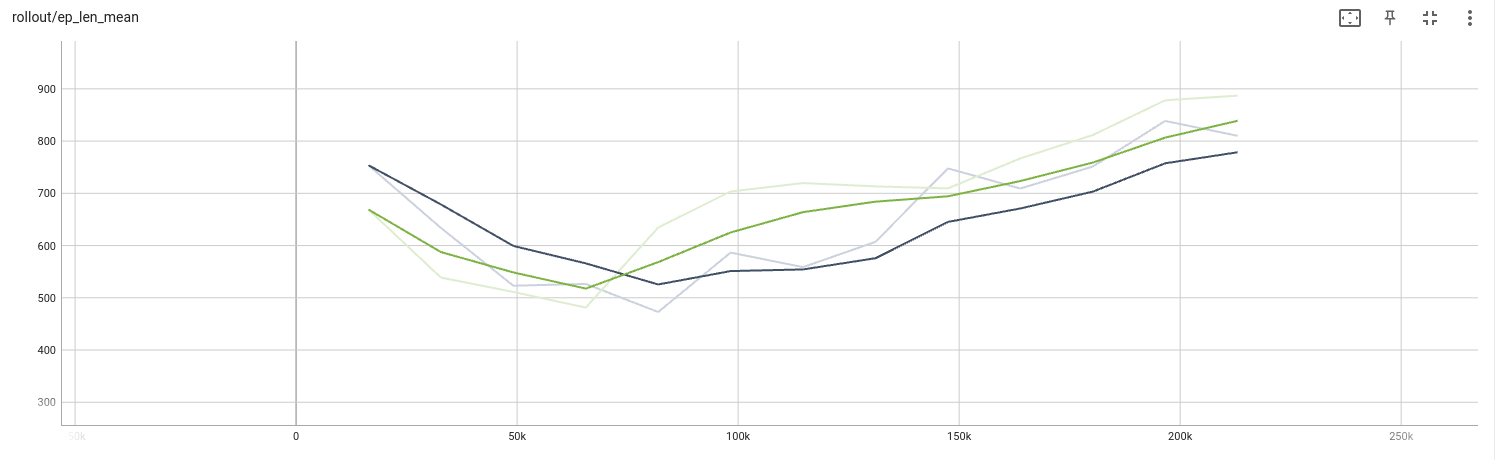
\includegraphics[width=1\linewidth]{Results/PPO_CNN/ep_length.png}
	\caption{ Episode Length}
	\label{f:g1}	
\end{figure}


\begin{figure}[ht]
	\centering
	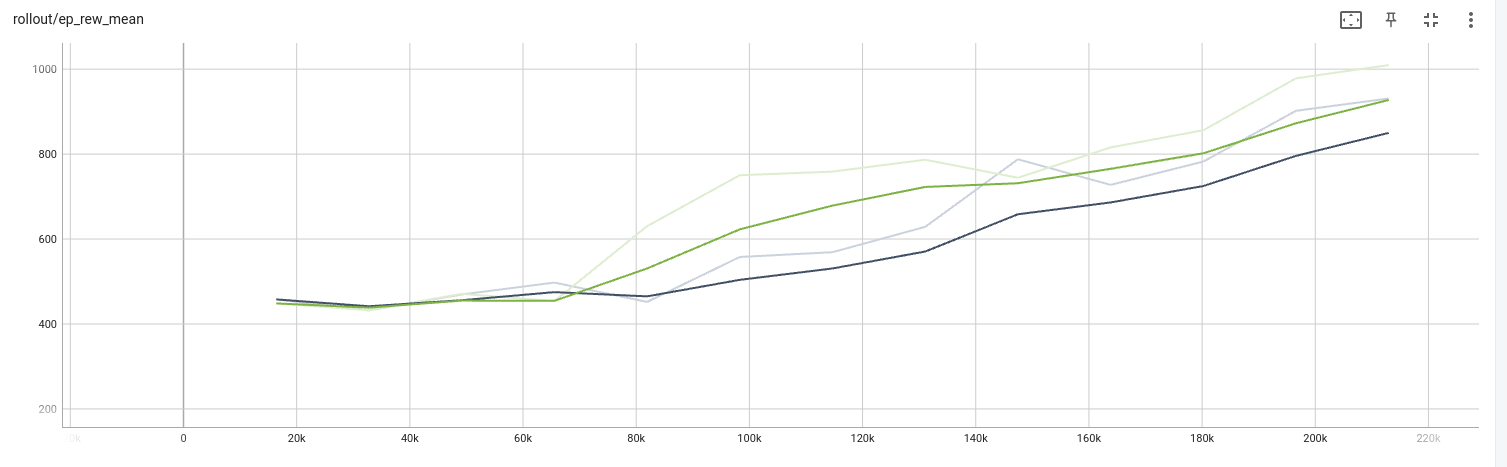
\includegraphics[width=1\linewidth]{Results/PPO_CNN/ep_reward.png}
	\caption{ Episode Reward }
	\label{f:g2}	
\end{figure}

\begin{figure}[ht]
	\centering
	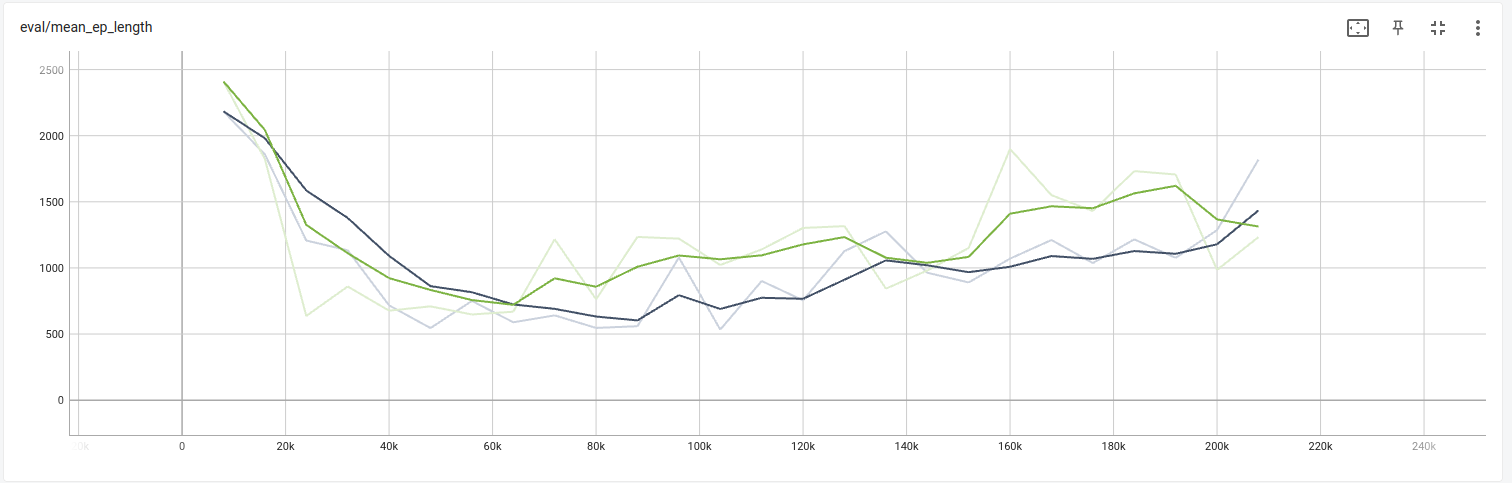
\includegraphics[width=1\linewidth]{Results/PPO_CNN/eval_length.png}
	\caption{ Evaluation Length}
	\label{f:g3}	
\end{figure}

\begin{figure}[ht]
	\centering
	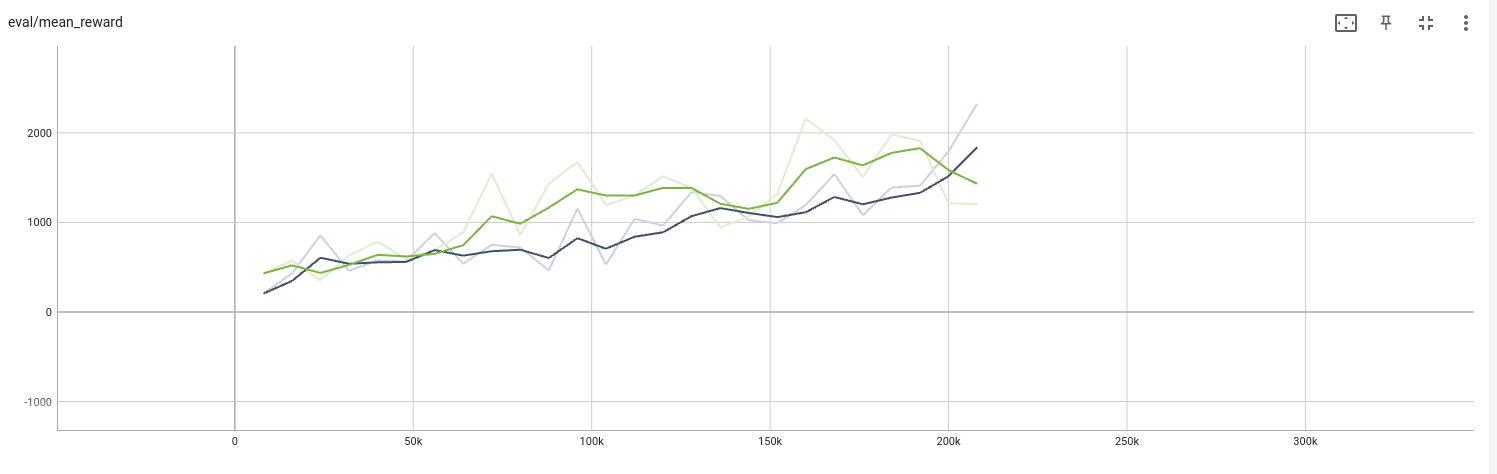
\includegraphics[width=1\linewidth]{Results/PPO_CNN/eval_reward.png}
	\caption{ Evaluation Reward}
	\label{f:g4}	
\end{figure}


\begin{figure}[ht]
	\centering
	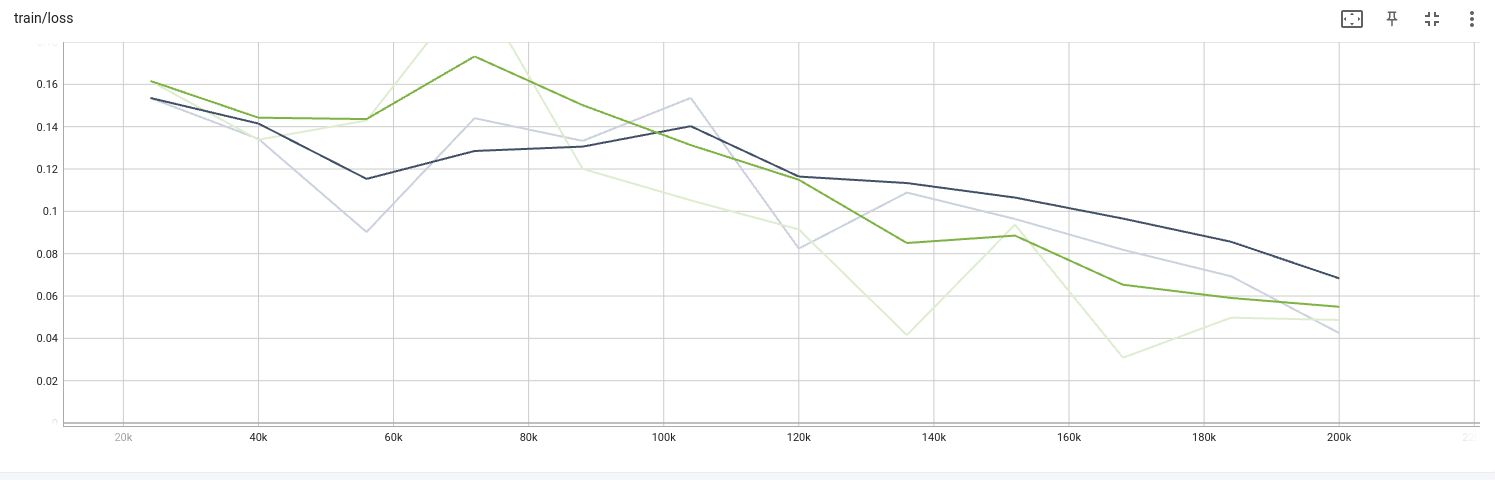
\includegraphics[width=1\linewidth]{Results/PPO_CNN/train_loss.png}
	\caption{Train loss}
	\label{f:g5}	
\end{figure}

\clearpage 


\subsection{Default MlpPolicy vs Custom MlpPolicy}

Στις δύο επόμενες εκπαιδεύσεις έχουν παραχθει τα παρακάτω 5 διαγράμματα \ref{f:g41}, \ref{f:g51}, \ref{f:g6}, \ref{f:g7} \ref{f:g8}, όπως και πιο πανω. Η μπλέ γραμμή αντιστοιχεί στο CustomMlpPolicy και η ροζ στο DefaultMlpPolicy. Στην συγκεκριμένη περίπτωση παρατηρούμε οτι 
το DefaultMlpPolicy παρόλο που έχει μεγαλύτερο reward και length στα τελευταία βήματα απο ότι το custom στο evalutation πέφτει πολύ πιο κάτω απο το episode. Αυτό οφείλεται σε overfitting(ίσως reverse exploration-exploitation trade-off) του default αφου η μεγιστη τιμή στο episode reward ειναι σχεδόν 800 ενώ στο evaluation οριακά φτάνει στο 500. Μεγαλύτερη διαφορά παρατηρείται αντίστοιχα μεταξυ episode length και evaluation length. Από την άλλη το custom στο evalutation ανεβαινει σχεδόν στο διπλασιο το reward του σε σχέση με το episode, τότε έχουμε exploration-exploitation-trade-off. Δηλαδή κατα την διάρκεια του training episode ο agent δοκιμάζει μόνο actions χωρίς να δίνει έμφαση στα policies που το βοηθάνε να σκοτώσει τους εχθρούς και να μαζέψει ποντους οπότε παιρνει χαμηλο reward και δεν διαρκεί πολυ το παιχνιδι. Απο την άλλη κατα την evaluation κατάσταση χρησιμοποιείται μόνο το exploitation των policies και έχει συνέχως μεγάλα rewards, κατι που παρατηρουμε και στα episode/reward lengths διαγράμματα \ref{f:g41}, \ref{f:g8}



\begin{figure}[ht]
	\centering
	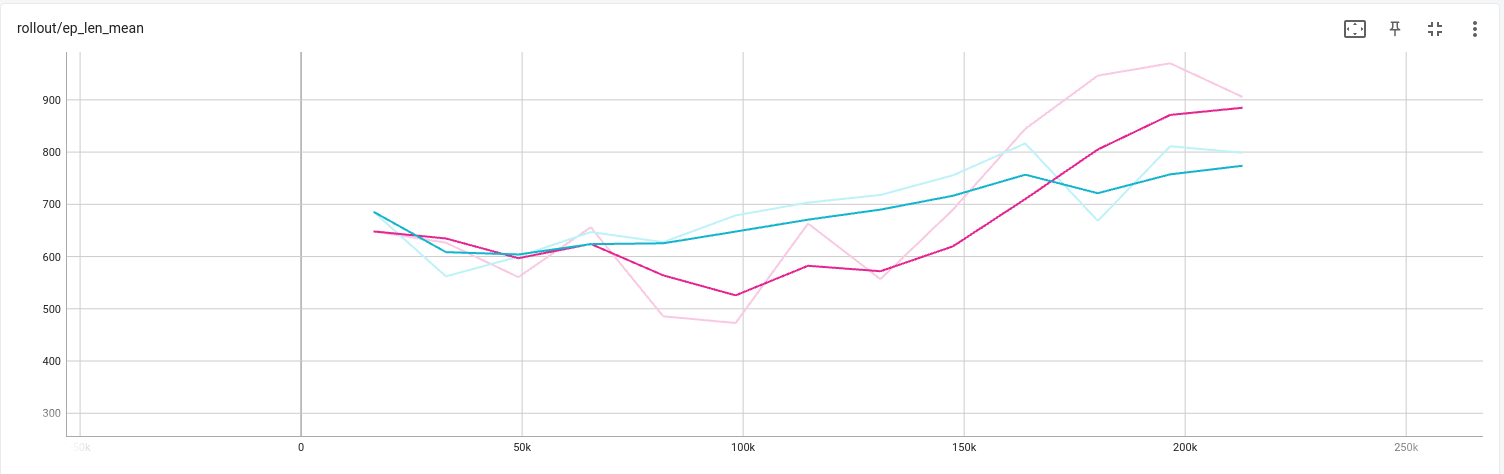
\includegraphics[width=1\linewidth]{Results/PPO_MLP/ep_length.png}
	\caption{ Episode Length}
	\label{f:g41}	
\end{figure}


\begin{figure}[ht]
	\centering
	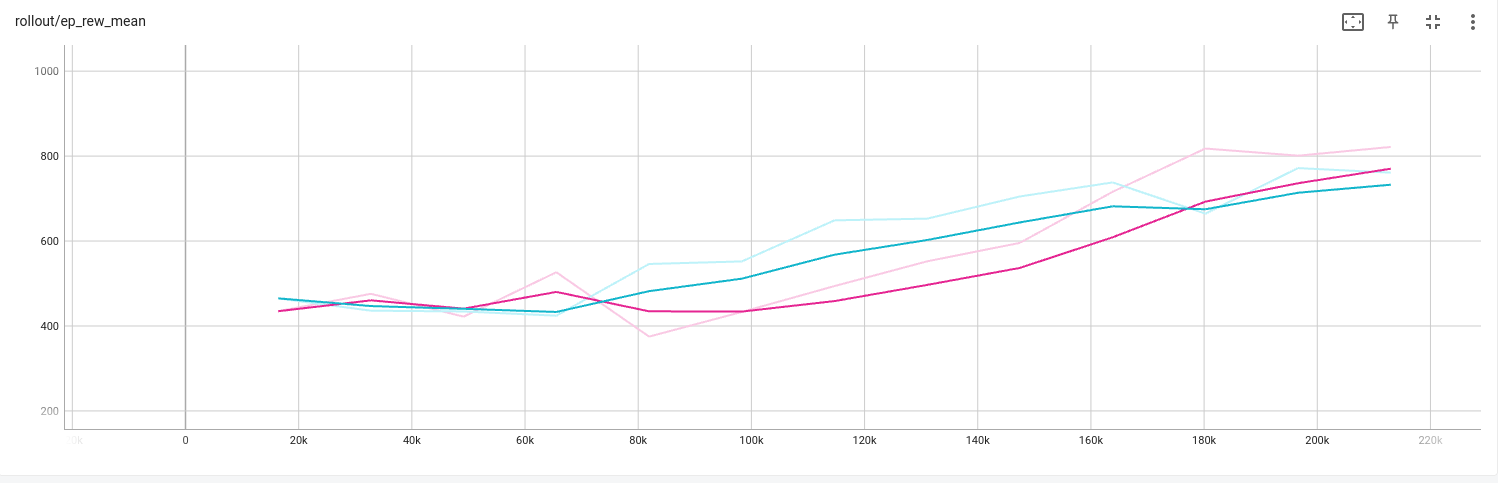
\includegraphics[width=1\linewidth]{Results/PPO_MLP/ep_reward.png}
	\caption{ Episode Reward }
	\label{f:g51}	
\end{figure}

\begin{figure}[ht]
	\centering
	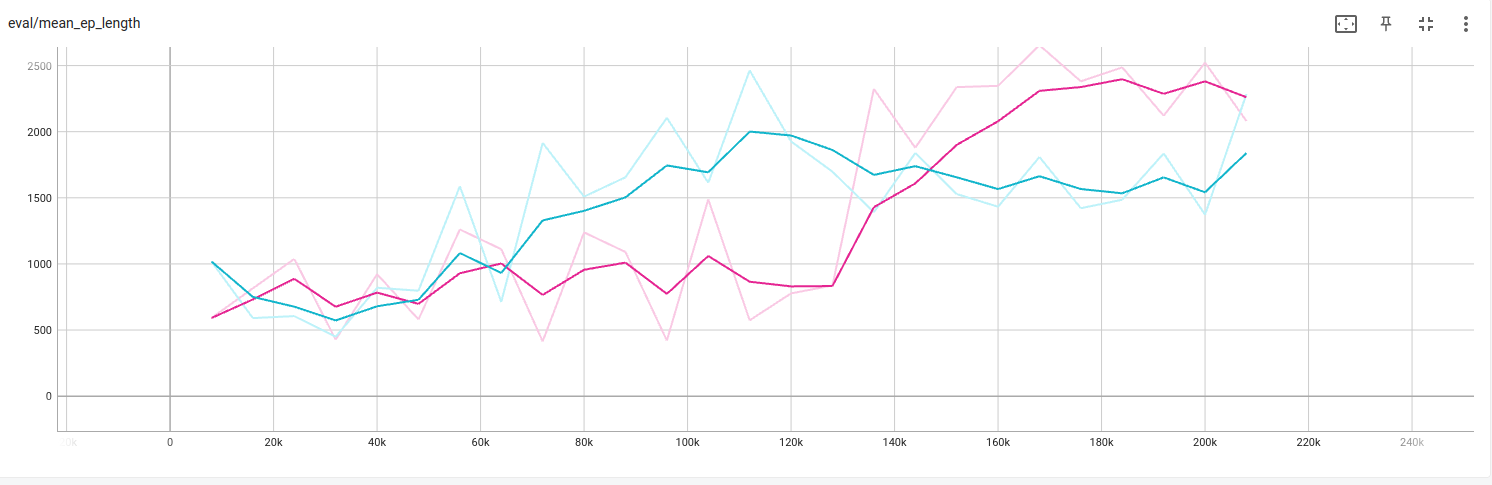
\includegraphics[width=1\linewidth]{Results/PPO_MLP/eval_length.png}
	\caption{ Evaluation Length}
	\label{f:g6}	
\end{figure}

\begin{figure}[ht]
	\centering
	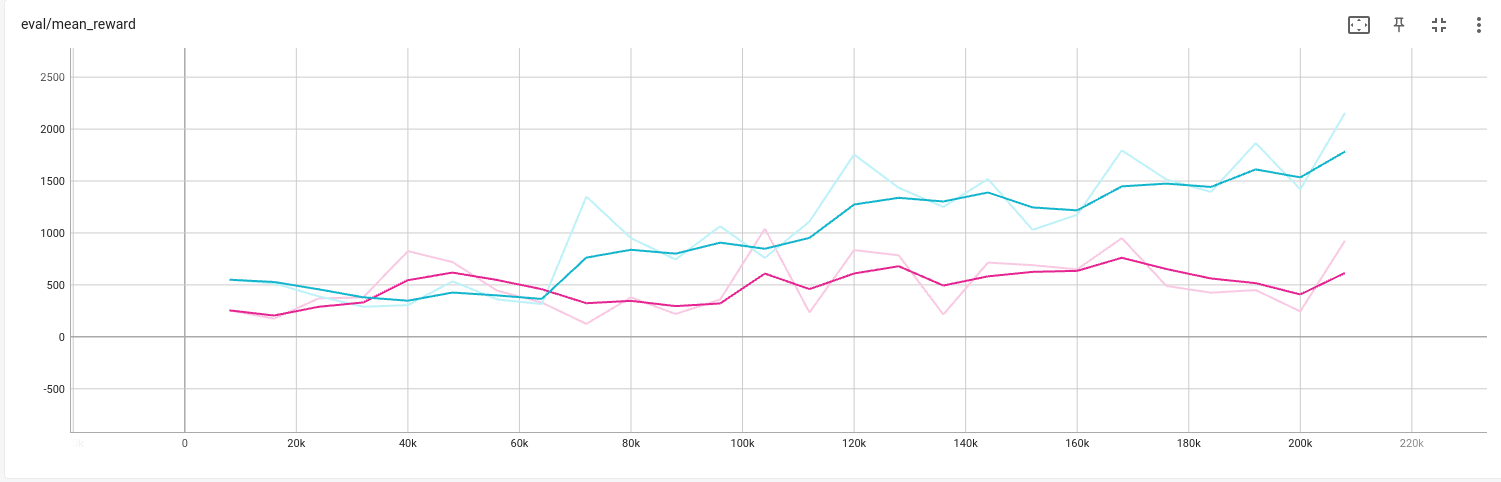
\includegraphics[width=1\linewidth]{Results/PPO_MLP/eval_reward.png}
	\caption{ Evaluation Reward}
	\label{f:g7}	
\end{figure}


\begin{figure}[ht]
	\centering
	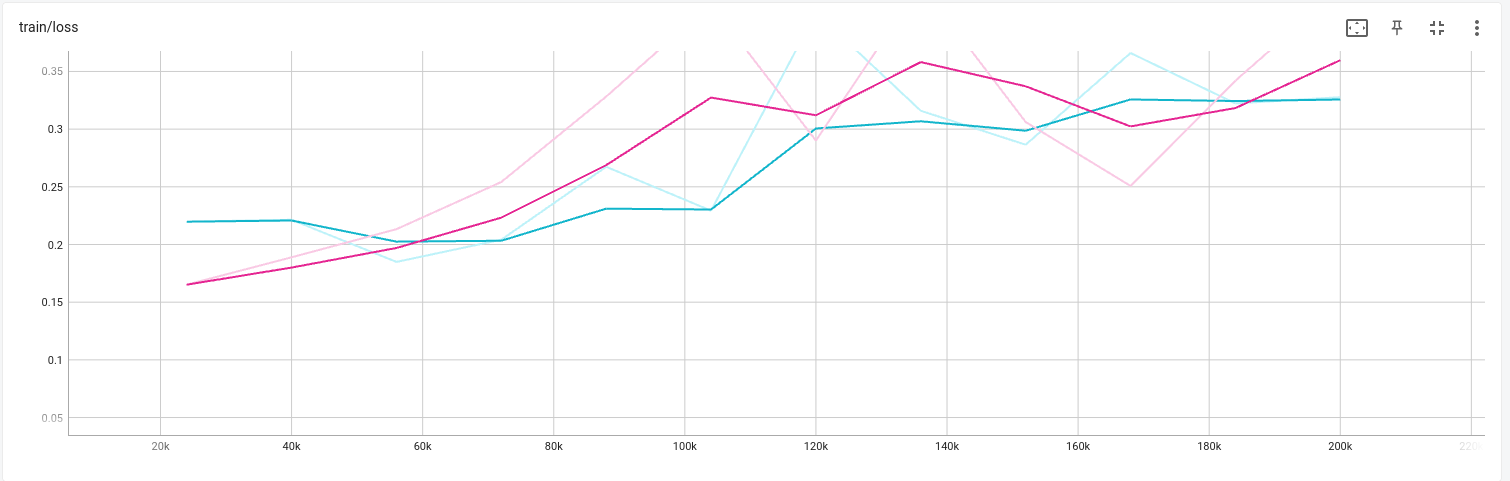
\includegraphics[width=1\linewidth]{Results/PPO_MLP/train_loss.png}
	\caption{Train loss}
	\label{f:g8}	
\end{figure}
\clearpage

\section{A2C Algorithm}
Με τον αλγόριθμο A2C έγιναν 4 εκαπιδέυσεις:

1. Η εκπαίδευση πραγματοποιήθηκε με CNNPolicy, xωρίς ορίσματα (defaultCNNPolicy).

2. Η εκπαίδευση πραγματοποιήθηκε με CNNPolicy και με όρισμα το CNN μοντέλο (customCNNPolicy).

3. Η εκπαίδευση πραγματοποιήθηκε με MlpPolicy χωρίς ορίσματα (defaultMlpPolicy) .

4. Η εκπαίδευση πραγματοποιήθηκε με MlpPolixy και με όρισμα το NN μοντέλο (customMlpPolicy).



\subsection{Default CNNPolicy vs Custom CNNPolicy}



Στις δύο πρωτες εκπαιδεύσεις έχουν παραχθεί τα παρακάτω 4 διαγράμματα \ref{f:g9}, \ref{f:g10}, \ref{f:g11}, \ref{f:g12}.
Η πορτοκαλί γραμμή αντιστοιχεί στο CustomCNNPolicy και η ροζ στο DefaultCNNPolicy. Παρατηρείται και εδώ στο DefaultCNNPolicy μοντέλο exploration-exploitation trade-off, αφού το evaluation reward ειναι 2000 ενώ το episode reward είναι κάτω απο 1000. Απο την άλλη ενώ το customCNNPolicy έχει χαμηλή απόδοση παραμένει παρόμοια και στα δύο περιβάλλοντα. Το episode length του σε κάποιες στιγμές φτάνει να είναι ίδιο με του Default που αυτο μας δίνει να καταλαβουμε οτι ο agent έχει μάθει να προσπαθεί στο ελάχιστο για να μην χάσει.






\begin{figure}[ht]
	\centering
	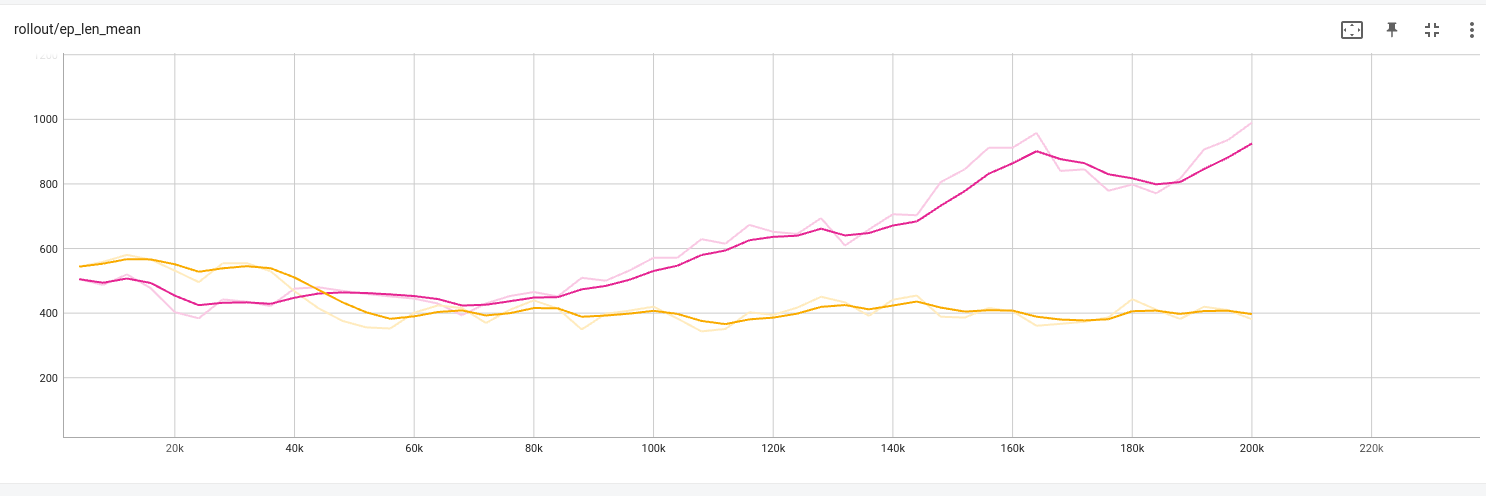
\includegraphics[width=1\linewidth]{Results/A2C_CNN/ep_length.png}
	\caption{ Episode Length}
	\label{f:g9}	
\end{figure}


\begin{figure}[ht]
	\centering
	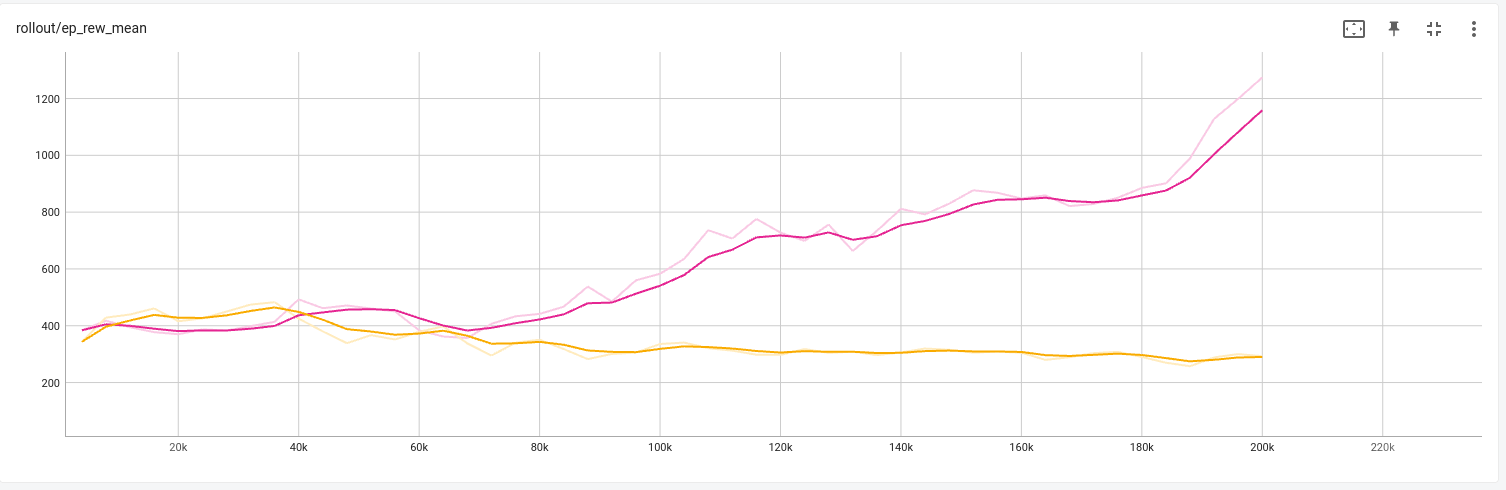
\includegraphics[width=1\linewidth]{Results/A2C_CNN/ep_reward.png}
	\caption{ Episode Reward }
	\label{f:g10}	
\end{figure}

\begin{figure}[ht]
	\centering
	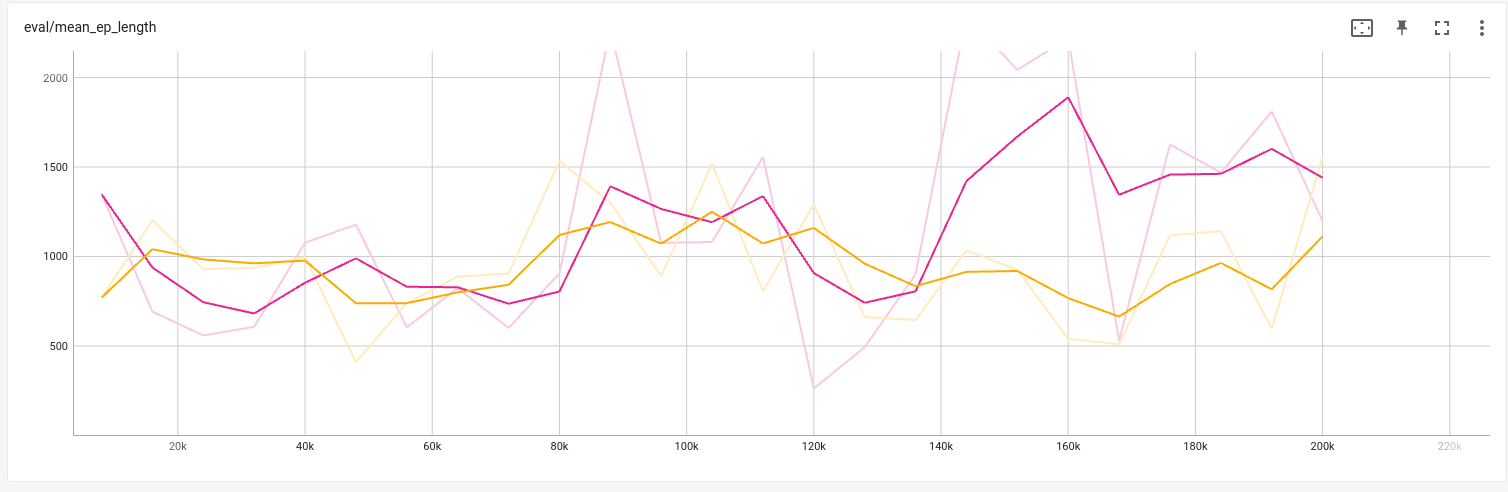
\includegraphics[width=1\linewidth]{Results/A2C_CNN/eval_length.png}
	\caption{ Evaluation Length}
	\label{f:g11}	
\end{figure}

\begin{figure}[ht]
	\centering
	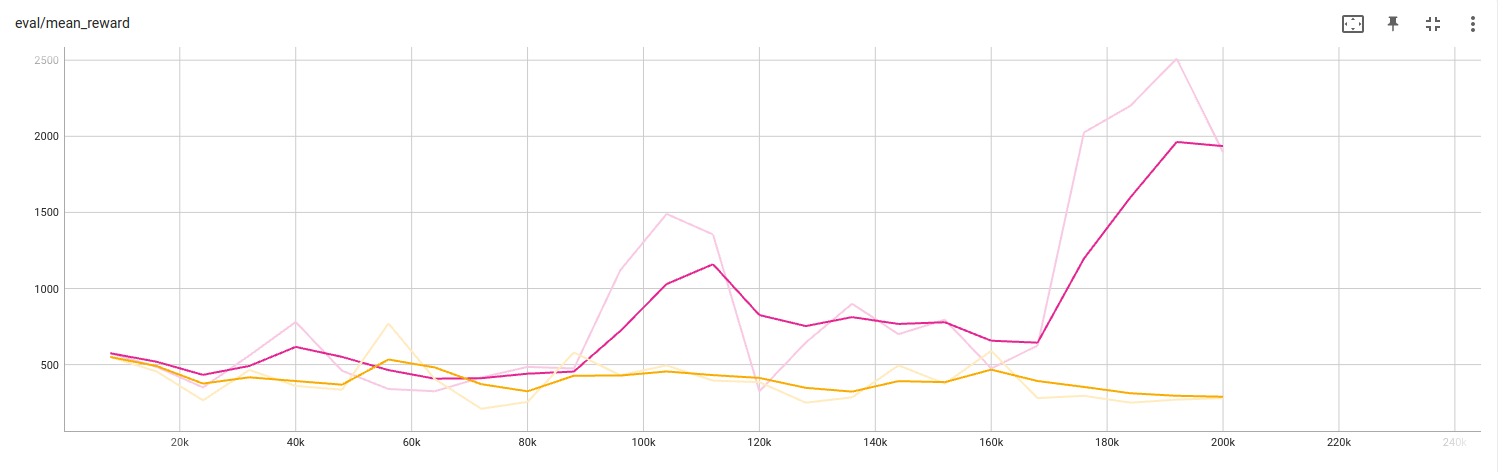
\includegraphics[width=1\linewidth]{Results/A2C_CNN/eval_reward.png}
	\caption{ Evaluation Reward}
	\label{f:g12}	
\end{figure}

\clearpage

\subsection{Default Mlpolicy vs Custom MlpPolicy}

Στις δύο επόμενες εκπαιδεύσεις έχουν παραχθεί τα παρακάτω 4 διαγράμματα \ref{f:g13}, \ref{f:g14}, \ref{f:g15}, \ref{f:g16}, όπως πιο πάνω.
Η μπλέ γραμμή αντιστοιχεί στο CustomMlp και η μάυρη αντιστοιχεί στο Default. Αυτό που παρατηρείται και στις δυο περιπτώσεις είναι οτι το length τόσο του evaluation όσο και του episode είναι παρα πολυ υψηλό σε σχεση με τα αντίστοιχα rewards. Αυτό μπορεί να οφείλεται
Exploration vs. Exploitation, Suboptimal Policy, Sparse Rewards :

Ο αλγόριθμος A2C εξισορροπεί το exploration (δοκιμή νέων ενεργειών) με το exploitation (επιλογή ενεργειών που είναι πιθανό να αποφέρουν υψηλές ανταμοιβές). Εάν το length είναι σταθερά υψηλότερο από το reward, αυτό μπορεί να υποδεικνύει ότι ο agent εξερευνά κυρίως το περιβάλλον και δεν εκμεταλλεύεται ακόμη τη βέλτιστη στρατηγική για τη μεγιστοποίηση των ανταμοιβών, και επειδή σταματάμε στα 200000 βήματα που είναι σχετικά μικρή τιμή για RL, δεν ξέρουμε αν μετά ανέβει το reward

Επίσης το customCNN μοντέλο που περνάει στο CNNPolicy ενδέχεται να μην μαθαίνει αποτελεσματικά τα υποκείμενα μοτίβα του παιχνιδιού. Η αρχιτεκτονική του μοντέλου, οι υπερπαράμετροι ή η διαδικασία εκπαίδευσης μπορεί να προκαλούν τo policy να παράγει ενέργειες που δεν ευθυγραμμίζονται με τη μεγιστοποίηση των rewards.

Τέλος τέτοιους είδους παιχνδίδια έχουν συνήθως sparse rewards signals, πράγμα που σημαίνει ότι ο agent λαμβάνει θετικά rewards σπάνια. Αυτό μπορεί να κάνει τη μάθηση πιο δύσκολη, καθώς ο agent μπορεί να δυσκολεύεται να συσχετίσει συγκεκριμένες ενέργειες με τις καθυστερημένα rewards. Σε τέτοιες περιπτώσεις, μπορεί να χρειαστεί περισσότερος χρόνος για να μάθει ο agent μια αποτελεσματική πολιτική που να επιτυγχάνει σταθερά υψηλά rewards.





\begin{figure}[ht]
	\centering
	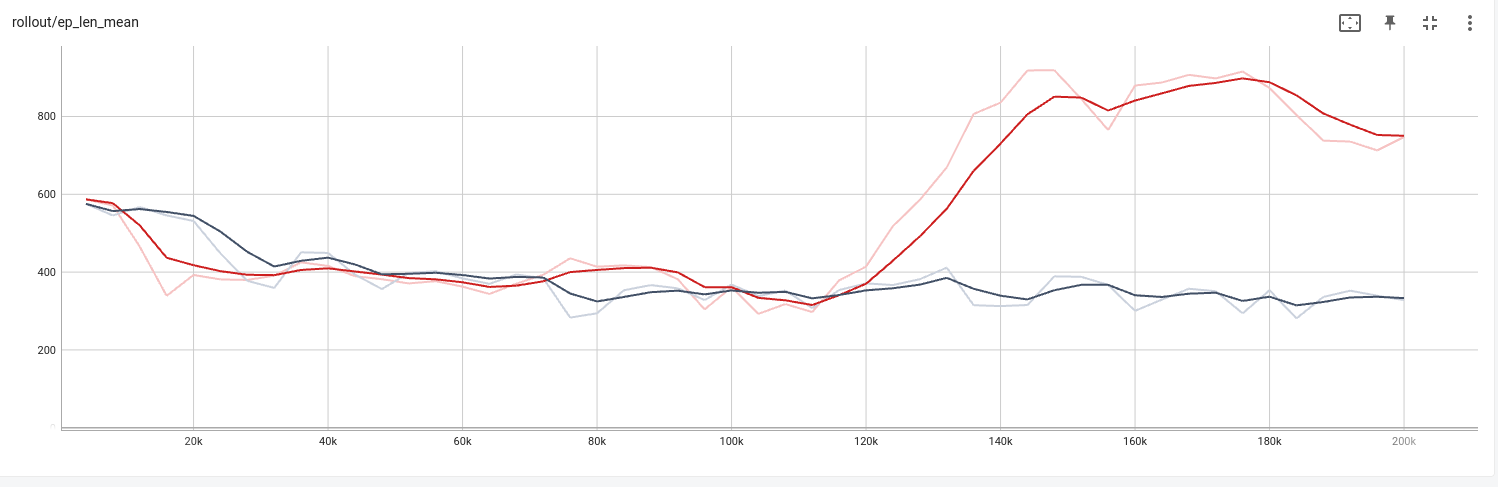
\includegraphics[width=1\linewidth]{Results/A2C_MLP/ep_length.png}
	\caption{ Episode Length}
	\label{f:g13}	
\end{figure}


\begin{figure}[ht]
	\centering
	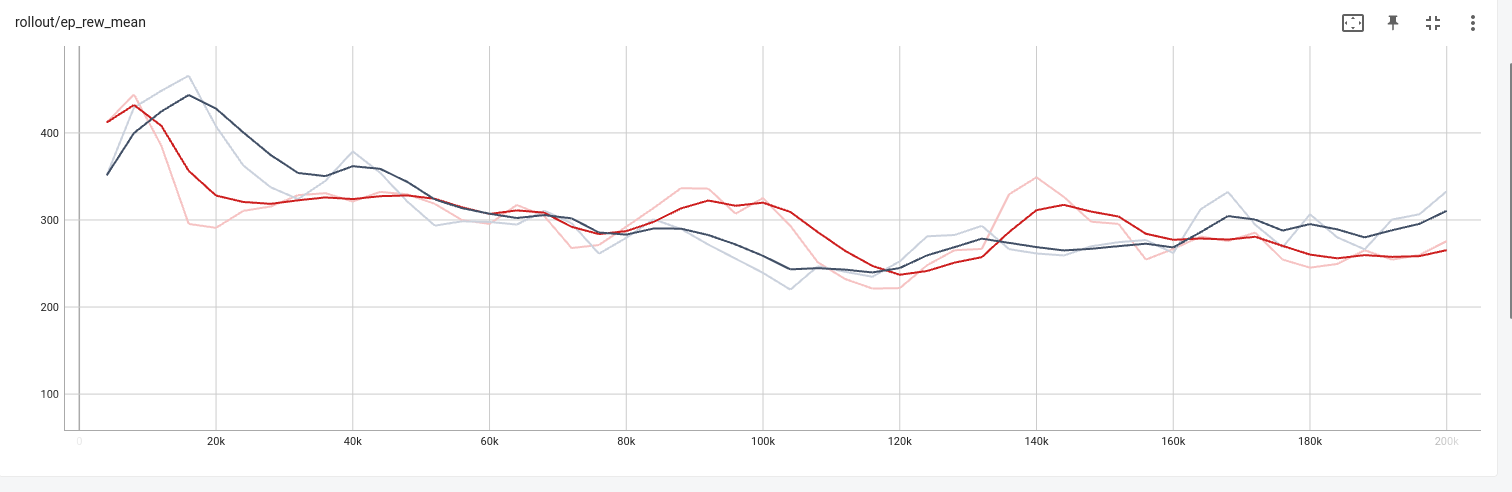
\includegraphics[width=1\linewidth]{Results/A2C_MLP/ep_reward.png}
	\caption{ Episode Reward }
	\label{f:g14}	
\end{figure}

\begin{figure}[ht]
	\centering
	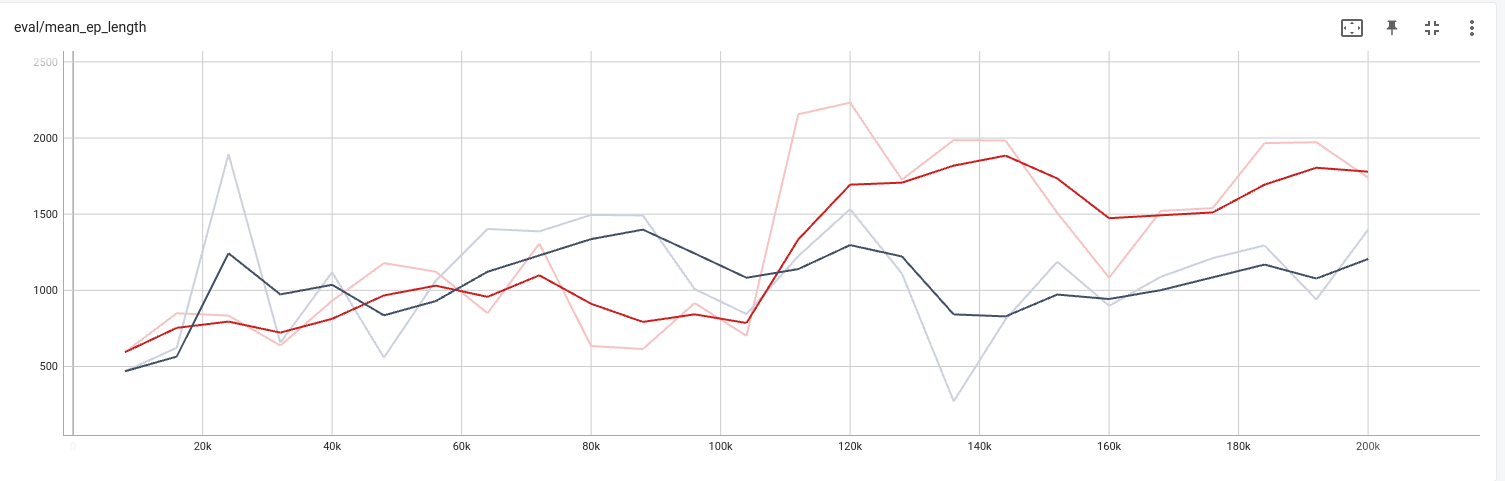
\includegraphics[width=1\linewidth]{Results/A2C_MLP/eval_length.png}
	\caption{ Evaluation Length}
	\label{f:g15}	
\end{figure}

\begin{figure}[ht]
	\centering
	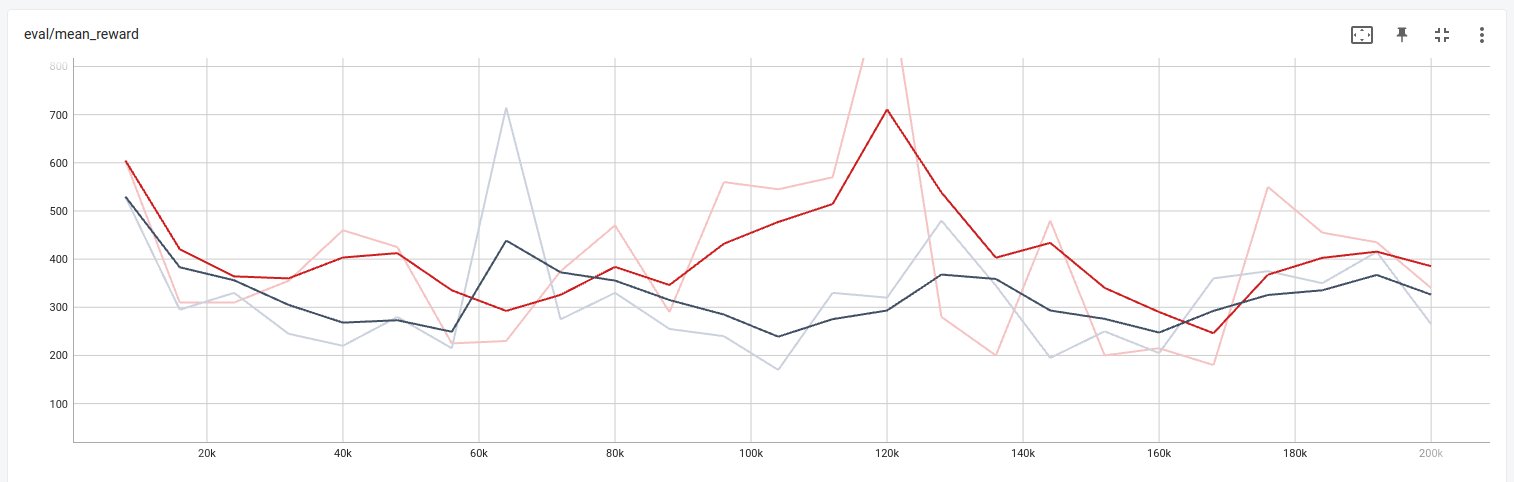
\includegraphics[width=1\linewidth]{Results/A2C_MLP/eval_reward.png}
	\caption{ Evaluation Reward}
	\label{f:g16}	
\end{figure}
\clearpage

\section{PPO vs A2C}

Στο τέλος συγκρίνουμε όλες τι εκπαιδεύσεις και παρατηρουμε στα δύο διαγράμμα \ref{f:g17}, \ref{f:g18}, ότι το A2C με defaultCNNPolicy έχει την καλύτερη απόδοση στο reward. Το PPO με customCNNPolicy στο episode reward διάγραμμα φαίνεται οτι έχει σταθερή αύξηση, ενώ στο evaluation reward διάγραμμα ξεκινάει στο τέλος να πέφτει. Τα δύο μοντέλα που έχουν σχετικά καλές αποδόσεις είναι τα PPO MLPCustomPolicy και PPO DefaultCnnPolicy, Τα υπόλοιπα μοντέλα είναι πιο ασταθή στην διάρκεια του χρόνου.

\begin{figure}[ht]
	\centering
	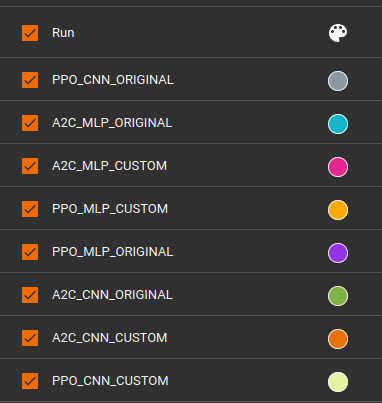
\includegraphics[width=0.4\linewidth]{Results/A2CvPPO/colors.png}
	\caption{ Color of the Models}
	\label{f:g19}	
\end{figure}

\begin{figure}[ht]
	\centering
	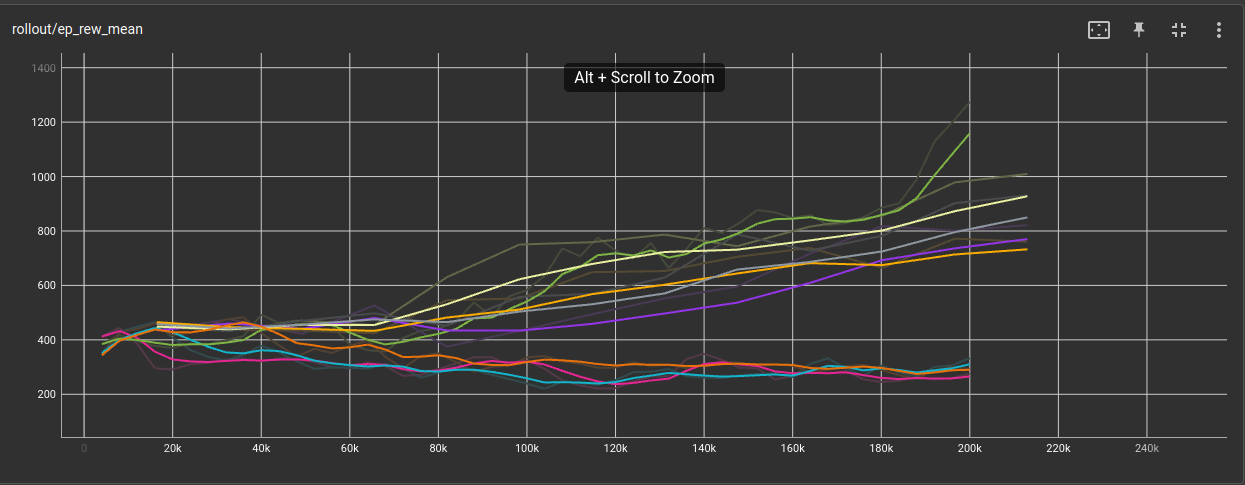
\includegraphics[width=1\linewidth]{Results/A2CvPPO/ep_reward.png}
	\caption{ Episode Reward }
	\label{f:g17}	
\end{figure}

\begin{figure}[ht]
	\centering
	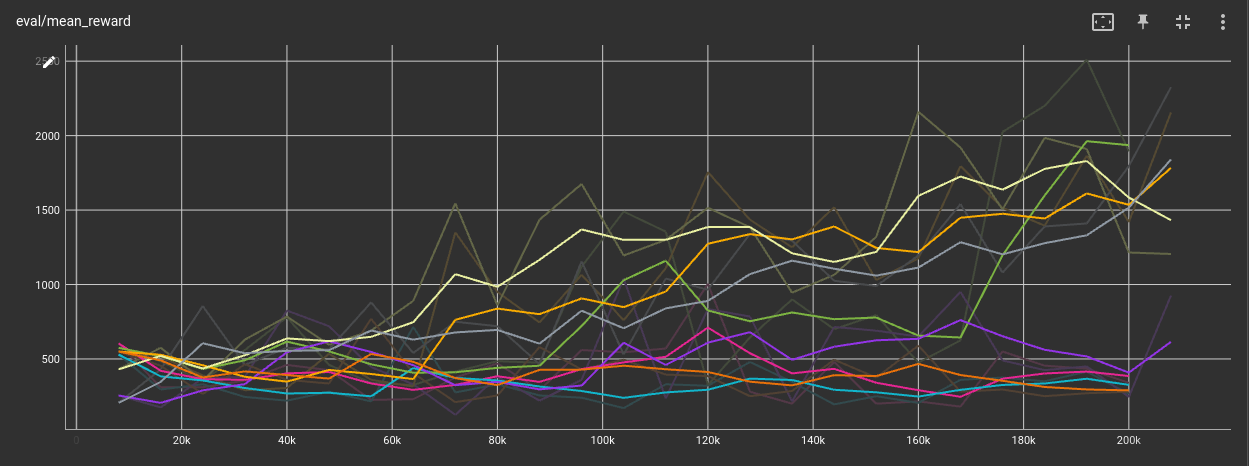
\includegraphics[width=1\linewidth]{Results/A2CvPPO/eval_reward.png}
	\caption{ Evaluation Reward}
	\label{f:g18}	
\end{figure}


